\documentclass[12pt,reqno]{amsart}

\usepackage{amsthm,amsmath,amssymb}
\usepackage{mathtools}
\usepackage{proof}
\usepackage{xcolor}
\usepackage{graphicx}
\usepackage[T1]{fontenc}
\usepackage{courier}
\usepackage{hyperref}
\hypersetup{
    hidelinks=true
}
\usepackage{array}
\usepackage{multirow}
\usepackage{listings}
\lstset{basicstyle=\ttfamily\tiny, columns=fullflexible, language=Python, morekeywords={logical_and, log, exp, dot, sqrt, ones, identity}}
\newcommand{\code}[1]{\texttt{#1}}
\newcommand\MyBox[2]{
  \fbox{\lower0.75cm
    \vbox to 1.7cm{\vfil
      \hbox to 1.7cm{\hfil\parbox{1.4cm}{#1\\#2}\hfil}
      \vfil}%
  }%
}
\graphicspath{ {./} }

\begin{document}

\begin{center}
\large\textbf{Assignment 3 \\ DASC521 Fall 2019} \\
\normalsize\textbf{Introduction to Machine Learning \\  Erhan Tezcan 0070881 \\ 28.10.2019} \\
\end{center}

\section{Task}
We are given 1000 images ($28\times28$ pixels $= 784$ pixels), each image belonging to one of 5 classes which are types of clothes. For the implementation, we mainly use methods specified in chapter 11.7.3 of the book ``Introduction to Machine Learning'' by Ethem Alpaydın. We will split the data in half, first 500 to be used for training and the remaining 500 to be used for testing.

\section{Implementation}
We are going to do Multiclass Classification using Multilayer Perceptrons. Our input layer consist of images, we have 20 neurons in our hidden layer and 5 neurons in the output layer, each corresponding to a class label. The hidden layer will have sigmoid as activation function:
\begin{equation}
\sigma(a) = \frac{1}{1 + e^{-a}}
\end{equation} 
The output layer will have softmax as activation function:
\begin{equation}
\sigma(z)_j = \frac{e^{z_j}}{\sum_{k=1}^{K}e^{z_k}}
\end{equation}

It is important to note that we do One-Hot Encoding to our labels before we proceed, so that we can compare them to our predictions. \\

As for the error function, we use:
\begin{equation}
\text{E}(w, v|X) = - \sum_t \sum_i \hat{y}_i^t \log y_i^t
\end{equation}

We will want to minimize this error. Our gradient functions are:
\begin{equation}
\Delta v_{ih} = \eta \sum_t (\hat{y}_i^t - y_i^t)z_h^t
\end{equation}
\begin{equation}
\Delta w_{hj} = \eta \sum_t \left[ \sum_i (\hat{y}_i^t - y_i^t)v_{ih} \right]z_h^t (1 - z_h^t) x_j^t
\end{equation}

Our loop has two termination conditions:
\begin{enumerate}
\item Maximum iteration count is reached.
\item The absolute difference between current objective value and last objective value is less than $\epsilon$.
\end{enumerate}

We plot how the error changes by iteration, and we get the result below: \\
\begin{centering}
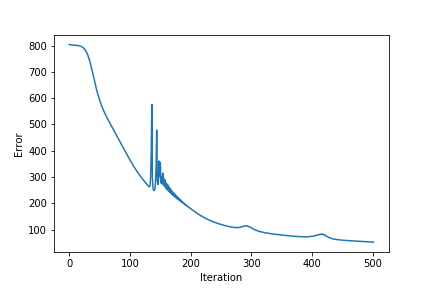
\includegraphics[width=0.6\textwidth]{test.png}
\end{centering}

Overall, our accuracies are: 
\begin{itemize}
\item Training Data: $97.2\%$
\item Test Data: $94.4\%$
\end{itemize}
\end{document}